\documentclass[12pt]{article}
\usepackage[T1, T2A]{fontenc}
\usepackage[utf8]{inputenc}
\usepackage[russian]{babel}
\usepackage{hyperref}
\usepackage{graphicx}
\graphicspath{ {../Images/} }

\author{Григорий Матюхин}
\date{\today}
\title{Лабораторная работа \textnumero12.\\Настройки сети в Linux}

\begin{document}
\maketitle
\newpage
\tableofcontents
\newpage
\section{Цель работы}
Получить навыки настройки сетевых параметров системы.

\section{Последовательность выполнения работы}

\subsection{Проверка конфигурации сети}
\begin{enumerate}
	\item Получите полномочия администратора.
	\item Выведите на экран информацию о существующих сетевых подключениях, а также статистику о количестве отправленных пакетов и связанных с ними сообщениях об ошибках:
	      \\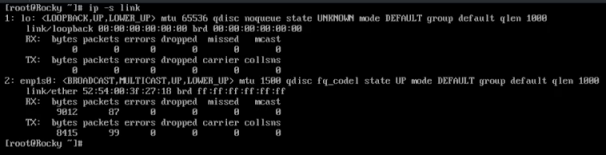
\includegraphics{1.png}
	\item Выведите на экран информацию о текущих маршрутах:
	      \\
\includegraphics{2.png}
	\item Выведите на экран информацию о текущих назначениях адресов для сетевых интерфейсов на устройстве:
	      \\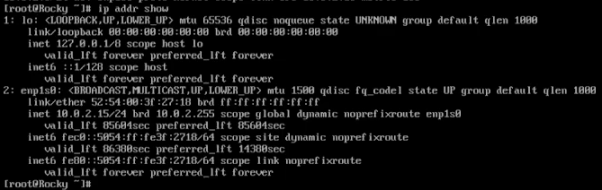
\includegraphics{3.png}
	\item Используйте команду \texttt{ping} для проверки правильности подключения к Интернету.
	      \\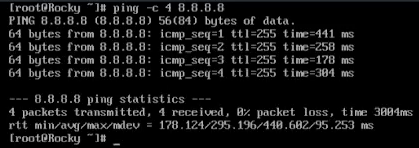
\includegraphics{4.png}
	\item Добавьте дополнительный адрес к вашему интерфейсу:
	      \\
\includegraphics{5.png}
	\item Выведите на экран список всех прослушиваемых системой портов UDP и TCP:
	      \\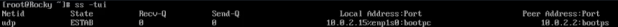
\includegraphics{6.png}
\end{enumerate}

\subsection{Управление сетевыми подключениями с помощью \texttt{nmcli}}
\begin{enumerate}
	\item Выведите на экран информацию о текущих соединениях:
	      \\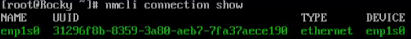
\includegraphics{7.png}
	\item Добавьте Ethernet-соединение с именем \texttt{dhcp} к интерфейсу:
	      \\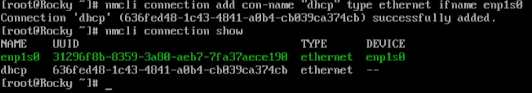
\includegraphics{8.png}
	\item Добавьте к этому же интерфейсу Ethernet-соединение с именем \texttt{static}, статическим IPv4-адресом адаптера и статическим адресом шлюза:
	      \\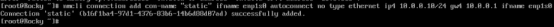
\includegraphics{9.png}
	\item Выведите информацию о текущих соединениях:
	      \\
\includegraphics{10.png}
	\item Переключитесь на статическое соединение:
	      \\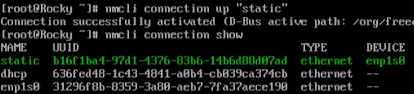
\includegraphics{11.png}
	\item Вернитесь к соединению \texttt{dhcp}:
	      \\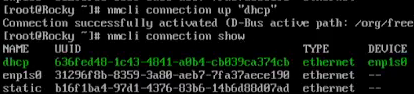
\includegraphics{12.png}
\end{enumerate}

\subsection{Изменение параметров соединения с помощью \texttt{nmcli}}
\begin{enumerate}
	\item Отключите автоподключение статического соединения:
	\item Добавьте DNS-сервер в статическое соединение:
	\item Добавьте второй DNS-сервер:
	\item Измените IP-адрес статического соединения:
	\item Добавьте другой IP-адрес для статического соединения:
	\item После изменения свойств соединения активируйте его:
	      \\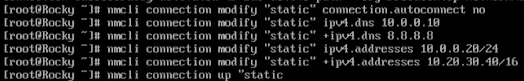
\includegraphics{13.png}
	\item Используя \texttt{nmtui}, посмотрите настройки сети на устройстве.
	      \\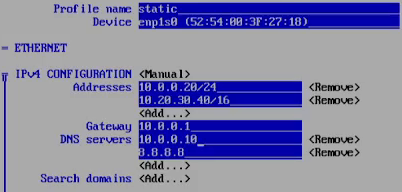
\includegraphics{14.png}
	\item Переключитесь на первоначальное сетевое соединение.
\end{enumerate}

\section{Контрольные вопросы}
\begin{enumerate}
	\item Какая команда отображает только статус соединения, но не IP-адрес? \\
	      \texttt{ip -s link}
	\item Какая служба управляет сетью в ОС типа RHEL? \\
	      \texttt{NetworkManager}
	\item Какой файл содержит имя узла (устройства) в ОС типа RHEL? \\
	      \texttt{/etc/hosts}
	\item Какая команда позволяет вам задать имя узла (устройства)? \\
	      \texttt{hostnamectl}
	\item Какой конфигурационный файл можно изменить для включения разрешения имён для конкретного IP-адреса? \\
	      \texttt{/etc/resolv.conf}
	\item Какая команда показывает текущую конфигурацию маршрутизации? \\
	      \texttt{ip route show}
	\item Как проверить текущий статус службы \texttt{NetworkManager}? \\
	      \texttt{systemctl status NetworkManager}
	\item Какая команда позволяет вам изменить текущий IP-адрес и шлюз по умолчанию для вашего сетевого соединения? \\
	      \texttt{nmcli connection modify "<name>" ipv4.addresses <new-address>}
\end{enumerate}


\section{Вывод}
В ходе выполнения данной работы я получил навыки настройки сетевых параметров системы.

\end{document}
